% results.tex
% Author: Tony Kabilan Okeke
% Date: 2023-03-23

\section{Experiments and Results}

Show your main findings.\\
Prefer figures (e.g., bar charts) over tables to pre-sent your results.\\
Compare your results to those from publications using these datasets. \\
This line refers to Figure \ref{fig:figure1}.\\
If you use tables to report your results, use References->Insert Caption->Table,
OnlyLabel\&Number to insert cross-reference to tables. E.g., See Table \ref{tab:table1}). \\
This line refers to Figure \ref{fig:figure2}.\\
Have something intelligible to say about each fig-ure/table you include.

    {
        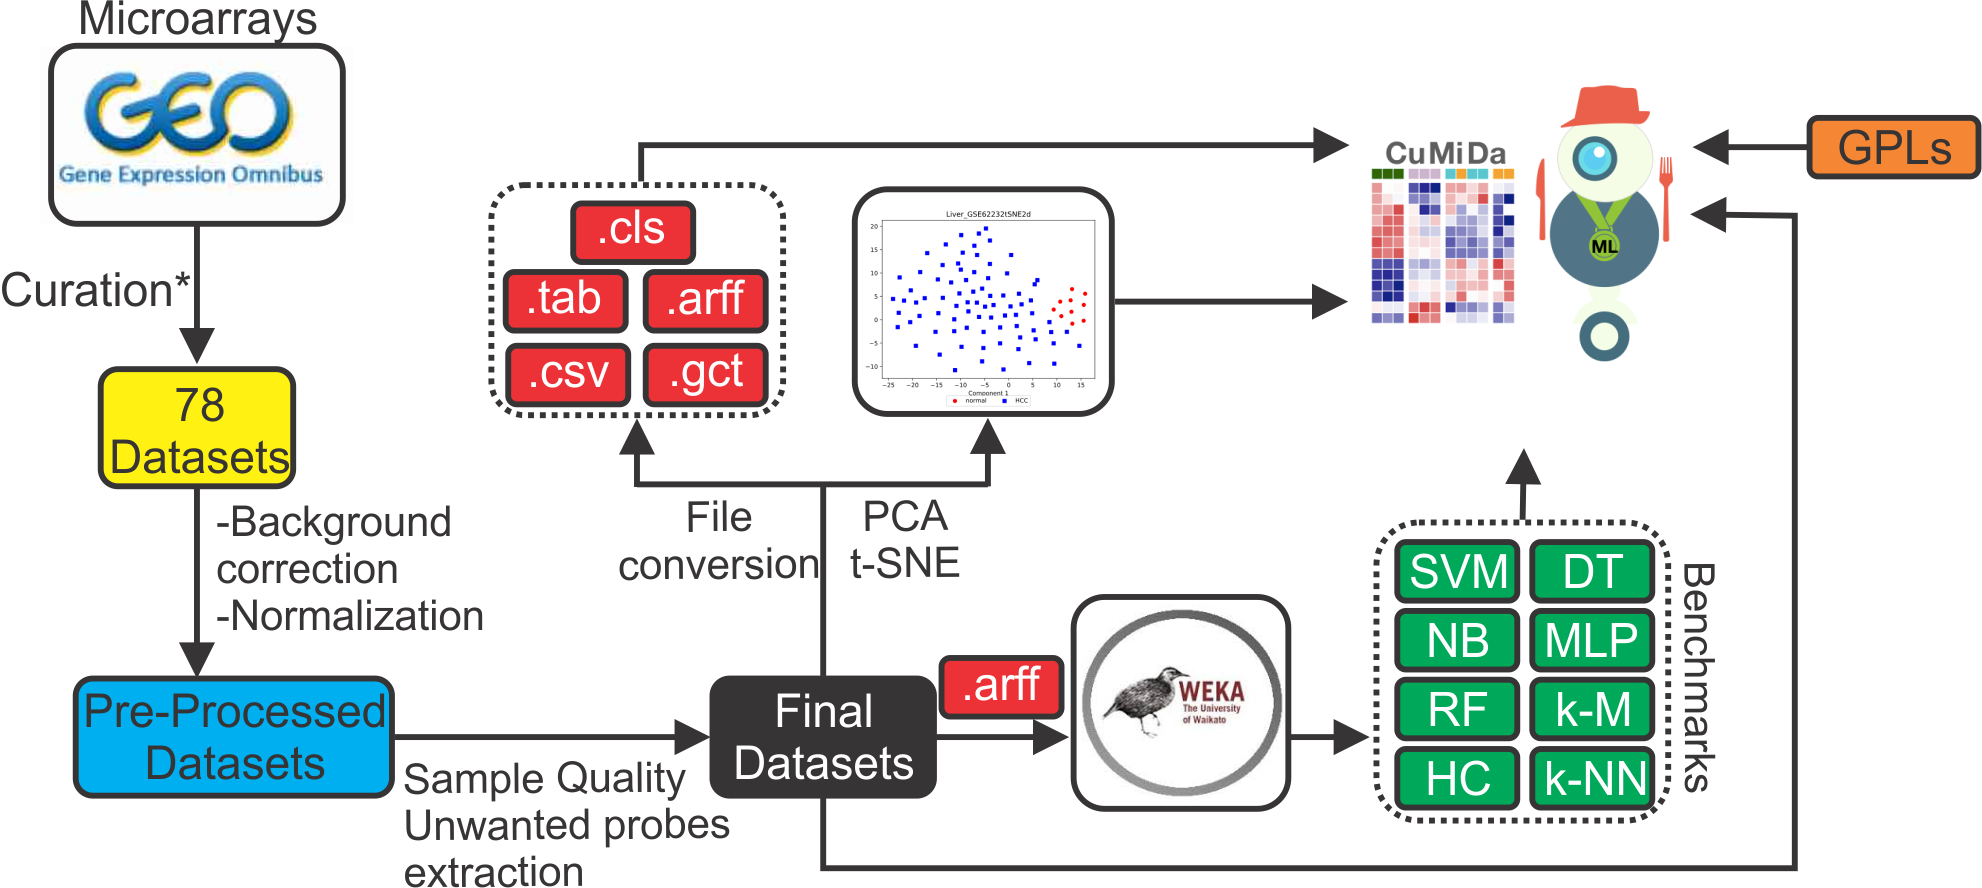
\includegraphics[width=\columnwidth]{./images/cumida.png}
        \captionof{figure}{A figure caption.}
        \label{fig:figure1}
    }

    {
        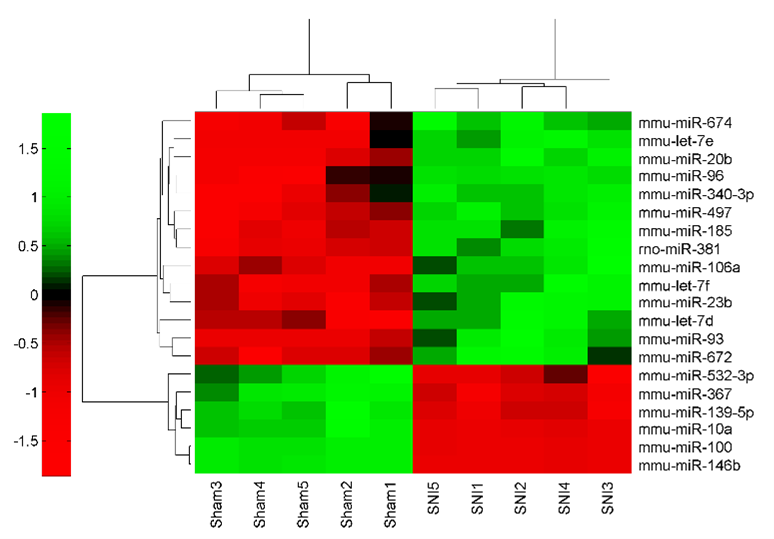
\includegraphics[width=\columnwidth]{./images/figure1.png}
        \captionof{figure}{A figure caption.}
        \label{fig:figure2}
    }

\begin{center}
    \begin{tabular}{l|r|r}
        \hline
        Name        & Fold Change & p-value \\
        \hline
        hsa-miR-25  & -3.9        & 1.1E-06 \\
        hsa-let-7c  & -2.5        & 2.1E-05 \\
        hsa-miR-939 & -4.6        & 5.6E-06 \\
        hsa-let-7a  & -2.5        & 0.002   \\
        hsa-let-7b  & -2.4        & 5.5E-05 \\
        \hline
    \end{tabular}
    \captionof{table}{A table caption.}
    \label{tab:table1}
\end{center}
